%%
%% This is file `squelette-rr.tex',
%% generated with the docstrip utility.
%%
%% The original source files were:
%%
%% RR.dtx  (with options: `sample')
%% ********************************************************************
%% Copyright (C) 1997-1999 2004 2006-2011 INRIA/APICS/MARELLE by Jose' Grimm
%% This file may be distributed and/or modified under the
%% conditions of the LaTeX Project Public License, either version 1.3
%% of this license or (at your option) any later version.
%% The latest version of this license is in
%%    http://www.latex-project.org/lppl.txt
%% and version 1.3 or later is part of all distributions of LaTeX
%% version 2003/12/01 or later.
%% An archive of the software can be found at
%%    ftp://ftp-sop.inria.fr/marelle/RR-INRIA

\documentclass[twoside]{article}
\usepackage[a4paper]{geometry}
\usepackage[latin1]{inputenc} % ou \usepackage[utf8]{inputenc}
\usepackage[T1]{fontenc} % ou \usepackage[OT1]{fontenc}
\usepackage{RR}
\usepackage{hyperref}
\usepackage{subfigure}
%%\usepackage[frenchb]{babel} % optionnel
\RRNo{7003}
%% \RTNo{0703}
%%
%% date de publication du rapport
\RRdate{April 2015}
%%
%% Cas d'une version deux
%% \RRversion{2}
%% date de publication de la version 2
%% \RRdater{November 2008}
%%
\RRauthor{% les auteurs
 % Premier auteur, avec une note
H\'el\'ene Coullon\thanks{Footnote for first author}%
  % note partag\'ee (optionnelle)
  \thanks[sfn]{Shared foot note}%
 % \and entre chaque auteur s'il y en a plusieurs
  \and
Christian Perez\thanks{Footnote for second author}%
 % r\'ef\'erence \`a la note partag\'ee
%\thanksref{sfn}
 % liste longue pour tests de mise en page
%\and Nicolas Bourbaki\thanks{etc} \and Andr\'e Lichnerowicz
%\and Marcel-Paul Sch\"utzenberger \and Jacques-Louis Lions
}
%% Ceci apparait sur chaque page paire.
\authorhead{Coullon \& Perez}
%% titre francais long
\RRtitle{Exemple de document\\
 utilisant le style\\rapport de recherche\\Inria}
%% English title
\RRetitle{Component-based implicit parallelism model for multi-stencil numerical simulations}
%%
%\titlehead{Example of RR.sty}
%%
%\RRnote{This is a note}
%\RRnote{This is a second note}
%%
\RRresume{Resume en francais
}
\RRabstract{
abstract }
%%
\RRmotcle{mots-cles}
%%
%% \RRprojet{Apics}  % cas d'un seul projet
\RRprojets{Avalon}
%%
%% \URLorraine % pour ceux qui sont \`a l'est
%% \URRennes  % pour ceux qui sont \`a l'ouest
%\URRhoneAlpes % pour ceux qui sont dans les montagnes
%% \URRocq % pour ceux qui sont au centre de la France
%% \URFuturs % pour ceux qui sont dans le virtuel
%% \URSophia % pour ceux qui sont au Sud.
%%
%% \RCBordeaux % centre de recherche Bordeaux - Sud Ouest
%% \RCLille % centre de recherche Lille Nord Europe
%% \RCParis % Paris Rocquencourt
%% \RCSaclay % Saclay \^Ile de France
 \RCGrenoble % Grenoble - Rh\^one-Alpes
%% \RCNancy % Nancy - Grand Est
%% \RCRennes % Rennes - Bretagne Atlantique
%\RCSophia % Sophia Antipolis M\'editerran\'ee
\newtheorem{mydef}{\textbf{Definition}}
\usepackage{amsmath}
\usepackage{amssymb}
\usepackage{graphics}
\usepackage{tikz}
\usepackage[ruled,noend]{algorithm2e}
\usetikzlibrary{calc,arrows,shapes,automata,petri,positioning,decorations.markings,shadows}

\tikzset{
    component/.style={
    rectangle,rounded corners=3pt,draw=black
    },
    smallcp/.style={
    rectangle,rounded corners=3pt,draw=black,font=\tiny,
    },
    resource/.style={
    rectangle,rounded corners=3pt, dashed,draw=black,font=\tiny,
    },
    connection/.style={
    decoration={ markings,
      mark=at position 1 with {\node[fill=black,draw=black,circle,,inner sep=2pt](conn){};}
      },
    postaction={decorate}
    },
    mpiconn/.style={
    decoration={ markings,
      mark=at position 0.99 with {\node[fill=black,draw=black,rectangle,,inner sep=2pt](mpi){};}
      },
    postaction={decorate}
    },
}


%%
\begin{document}
%%
\makeRR   % cas d'un rapport de recherche
%% \makeRT % cas d'un rapport technique.
%% a partir d'ici, chacun fait comme il le souhaite
%------------------------------------------------------------------------------
\section{Introduction}
\label{sect:introduction}
%------------------------------------------------------------------------------
\section{Stencil programs}
\label{sect:formalism}
To numerically solve a set of PDEs, iterative methods (finite difference, finite volume or finite element methods) are frequently used to approximate the solution through a discretized (step by step) phenomena. Thus, the continuous time and space domains are discretized so that a set of numerical computations are iteratively (time discretization) applied onto a mesh (space discretization). In other words, the PDEs are transformed to a set of numerical computations applied at each time step on elements of the discretized space domain. Among those numerical computations are found a set of numerical schemes, also called \textit{stencil computations}, a set of auxiliary computations also called \emph{local computations}, and finally a set of \emph{reductions} to reduce a bunch of values to a single scalar value.
This section gives formal definitions of what we call a \textit{stencil program} and its computations. Then, the different mid-grain parallelization techniques which can be applied on such program, are presented.

We denote stencil kernels discretized explicit numerical schemes which involve neighborhood computations, whatever the type of space discrtization is (mesh).

%-------------------------------------
\subsection{Time, mesh and data}

$\Omega=\mathbb{R}^n$ is the continuous space domain of a numerical simulation. %For example, if $n=3$, any geographic point on earth could be represented in this space in a given geographic coordinate system.
A mesh $\mathcal{M}$ defines the discretization of the continuous space domain $\Omega$ of a set of PDEs and is defined as follows.

\begin{mydef}
A mesh is a connected undirected graph $\mathcal{M}=(V,E)$, where $V\subset \Omega$ is the set of vertices and $E\subseteq V^2$ the set of edges. The set of edges $E$ of a mesh $\mathcal{M}=(V,E)$ does not contain bridges. It is said that the mesh is applied onto $\Omega$.
\end{mydef}
\begin{figure}[!h]\begin{center}
  \resizebox{8cm}{!}{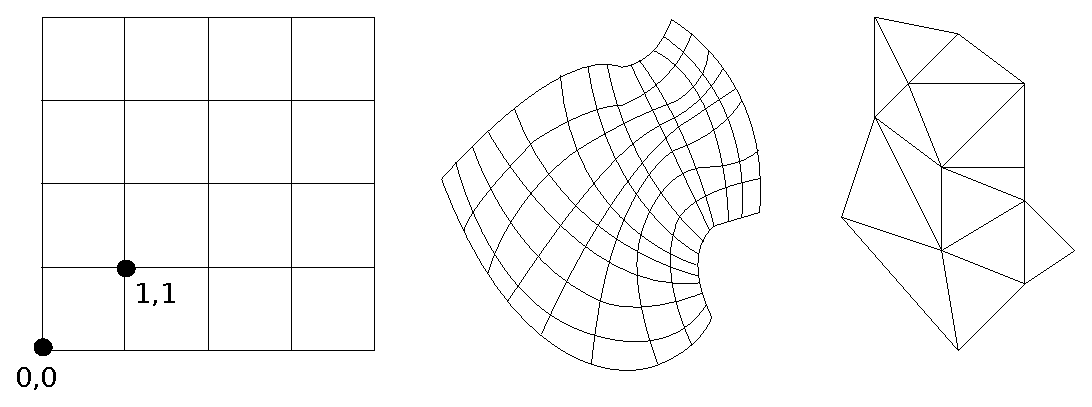
\includegraphics{./images/maillages.pdf}}
  \caption{From left to right, Cartesian, curvilinear and unstructured meshes.}
  \label{fig:mesh}
\end{center}\end{figure}
\begin{mydef}
The dimension of a mesh $\mathcal{M}=(V,E)$ applied onto $\Omega=\mathbb{R}^n$ is denoted $dim(\mathcal{M})=n$.
\end{mydef}
A mesh can be structured (as Cartesian or curvilinear meshes), unstructured, regular or irregular (without the same topology for each element) and hybrid as illustrated in Figure~\ref{fig:mesh}.

\medskip
\noindent \textbf{Definitions}
%\begin{mydef}
\begin{itemize}
\item An entity $e$ of a mesh $\mathcal{M}=(V,E)$ is defined as a subset of its vertices and edges, $e\subset V\cup E$.
\item A group of mesh entities is denoted $E$ such that $E \in \mathcal{P}(V\cup E)$. It represents a set of entities of the same type.
\item The set of mesh entities groups of a simulation is denoted $\mathcal{E}$.
\item Finally, the mesh on which is applied a group of mesh entities $E$ is denoted $mesh(E)$
\end{itemize}
%\end{mydef}

For example, in a 2D Cartesian mesh an entity could be a cell, made of four vertices and four edges, or simply a vertex. As a result, a group of cells and a group of vertices could be defined in $\mathcal{E}$. %This type can be defined as the sets containing exactly four vertices and four edges connected as a cycle. Another type of entities simply are the vertices ($V$) and can be defined as all singletons formed of a single vertex of $V$.

\medskip
This covers the space discretization, however there is also the time dimension which has to be discretized in the simulation.

\medskip
\noindent \textbf{Definitions}
%\begin{mydef}
\begin{itemize}
\item We denote a scalar as an identifier associated to a numerical value and applied onto a mesh $\mathcal{M}$ where $dim(\mathcal{M})=0$. In other words a scalar can be seen as a variable containing a numerical value. The set of scalars is denoted $\mathcal{S}$.
\item $\mathcal{T}=\mathbb{R}$ is the continuous time domain of a numerical simulation.
\item The discretization of the continuous time domain $\mathcal{T}$ is denoted as the pair $T(\Delta t,conv)$.
\begin{itemize}
\item $\Delta t \in \mathcal{S}$ represents the time interval of the numerical simulation, such that for a current time iteration $t_i$, the next time iteration is $t_{i+1} = t_i + \Delta t$. The default value of $\Delta t$ is $1$.
\item $conv:\mathcal{S}^n \rightarrow bool$ is a function which returns a boolean from a set of scalar variables. This function represents the convergence criteria of the simulation. 
\item At a given time step, the convergence criteria is evaluated such that if $conv$ returns $true$ the next time step can start such that $t_{i+1} = t_i + \Delta t$, otherwise the simulation ends. For example, the simplest $conv$ is typically to have two scalars: $t$ the time, and a fix number of iterations denoted $it$. At each time step $\Delta t=1$, and $conv$ returns the boolean expression $t<it$.
\end{itemize}
\end{itemize}
%\end{mydef}

%$T$ is responsible for the iteration time steps of the numerical simulation. A numerical simulation though does not run forever and must be stopped at some point. Some simulations choose a fix number of time iteration, others compute a \emph{convergence} criteria at the end of each time iteration to determine if the simulation has to continue. A convergence criteria is computed by a reduction computation that will be detailed in the next section.

In a numerical simulation, as a set of scalars can be applied onto a mesh with a nil dimension, a set of data elements, or quantities, can be applied onto meshes of dimension superior to zero. Those quantities represent, as well as scalars, the set of values to compute, or to use, for computations.

\medskip
\noindent \textbf{Definitions}
%\begin{mydef}
\begin{itemize}
\item A quantity (or data) is a function $\delta: E_{\delta} \mapsto V_{\delta}$ which associates each entity of a group $e\in E_{\delta}$ to a value $v\in V_{\delta}$ where $V_{\delta}$ is a primitive data type, typically $\mathbb{R}$, $\mathbb{N}$ or $\mathbb{C}$.
\item The set of quantities applied onto the mesh is denoted $\Delta$.
\item In the rest of this paper, the group of mesh entities on which a quantity $\delta$ is mapped is denoted $entity(\delta)=E_{\delta}$.
\end{itemize}
%\end{mydef}

Another option, closer to the applied mathematics domain, would have been to define $\delta$ as the function over $E_{\delta} \times T$. In this case a single quantity would represents all its occurences over time steps. This solution could be investigated in future work, however the approach chosen for now is to let the user be aware of the number of data he is using and what exactly for.

%-----------------------
\subsection{Computations}

In this section are considered four different types of kernel computations, stencil kernels, boundary kernels, local kernels, and reduction kernels. 

\medskip
\noindent \textbf{Definitions}
%\begin{mydef}
\begin{itemize}
\item A computation domain $D$ is a subpart of a mesh entities group, $D \subseteq E \in \mathcal{E}$.
\item The set of computation domains of a numerical simulation is denoted $\mathcal{D}$.
\item A neighborhood $n$ is a function which for a given entity $e \in E_i$, returns a set of $m$ entities in $E_j$, $n : E_i \rightarrow E_j^m$. One can notice that $i = j$ is possible. Most of the time, such a neighborhood is called a stencil shape.
\item The set of neihborhood functions in a numerical simulation is denoted $\mathcal{N}$.
\end{itemize}

\begin{mydef}
A computation kernel $k$ of a numerical simulation is defined as $k(S,R,(w,D),comp)$, where 
\begin{itemize}
\item $S \in \mathcal{S}$ is the set of scalar to read, 
\item $(w,D) \in \Delta \times \mathcal{D}$ is the single data modified by the computation kernel onto a given computation domain. Thus, $w \in \Delta$ and $D \in \mathcal{D}$ is the computation domain on which $w$ is computed, $D \subseteq E_w=entity(w)$.
\item $R$ is the set of tuples $(r,n)$, where $r \in \Delta$ and $n \in \mathcal{N}$ is a neighborhood function such that $n : E_w \rightarrow entity(r)^m$. The neighborhood indicates which entities of $r$ will be read in order to compute a single entity of $w$. 
\item $comp$ is the numerical computation which returns a value from a set of $n$ input values, $comp: V^n \rightarrow V$.
\end{itemize}
% \item A numerical expression $\text{exp}_{w}: entity(w) \times R^n \rightarrow V_{w}$ is a function which computes the values of the written quantity $w \in \Delta$ for a given entity $e \in entity(w)=E_w$, using a set of input data $R$.
% \item A computation kernel $k$ of a numerical simulation is defined as $c(R,w,\text{exp},D)$, where $R$ is the set of data read, $w \in \Delta$ is the unique data written, $\text{exp}$ is a numerical expression, and $D \in \mathcal{D}$ is the computation domain.
% \end{itemize}
%$R$ is the set of data read, $w \in \Delta$ is the unique data written, $\text{exp}$ is a numerical expression, and $D \in \mathcal{D}$ is the computation domain.
\end{mydef}

$comp$ represents the actual numerical expression which is computed by a kernel. We can dissociate four types of kernel computations.

\noindent \textbf{Definitions}
%\begin{mydef}
\begin{itemize}
\item We denote by $identity$ the identity function $x=x$.
\item A kernel computation $k(S,R,(w,D),comp)$ is a \emph{stencil kernel} $\iff \exists (r,n) \in R$ such that $n \neq identity$ and if $\exists (r,n)$ with $r=w$ then $n=identity$.
\item A kernel computation $k(S,R,(w,D),comp)$ is a \emph{boundary kernel} $\iff \exists (r,n) \in R$ such that $r=w$ and such that $n \neq identity$.
\item A kernel computation $k(S,R,(w,D),comp)$ is a \emph{local kernel} $\iff \forall (r,n) \in R$, $n = identity$.
\item A kernel computation $k(S,R,(w,D),comp)$ is a \emph{reduction kernel} $\iff w$ is a scalar, $R=\{(r,n)\}$, and if $n=entity(r)$.
\end{itemize}

In our formalism, it is forbidden for a stencil kernel to find $(r,n) \in R$ for which $r=w$ and $n \neq identity$. Actually, if such a property was permitted, implicit numerical schemes would be needed into the simulation, which involves linear solvers. Such a scheme is not a stencil and is over the scope of this paper. The problem does not happened for local kernels as $\forall (r,n) \in R$, $n = identity$. Computations for which this property is authorized are boundary kernels only. This type of kernel is a particular case as it commputes boundary conditions, which represents what should happened outside the space domain but still impact stencil kernels at the next time step.

\noindent \textbf{Property}
A kernel for which all data read and written are applied onto a mesh of dimension $0$ is a local kernel.

\noindent \textbf{Property}
In a reduction kernel $k(S,R,(w,D),comp)$, $D=entity(w)$ as a single entity exists for a scalar.

\medskip
A reduction computation is a computation which reads a single data applied onto a mesh and returns from all its entities a single scalar (mesh with a dimension reduced to zero). A reduction is typically used to compute the convergence criteria of the time loop of the simulation. Occasionally reductions can also be used during a time iteration. %This last usage is typically done to have a conditionnal branch to choose one computation or another, or to compute a dynamic time step for example.

\medskip
\noindent \textbf{Property}
Considering a reduction kernel $k(S,R,(w,D),comp)$, $comp$ must be a binary and associative operation on the type $V$, $comp: V \times V \rightarrow V$.

\medskip
\noindent \textbf{Definitions}
\begin{itemize}
\item The set of $n$ ordered computation kernels of a numerical simulation is denoted $\Gamma = [k_i]_{0 \leq i \leq n-1}$, such that $\forall k_i,k_j \in \Gamma$, if $i < j$, then $k_i$ is computed before $k_j$.
\item Finally, a \textit{multi-stencil program} is defined by the octuplet 
\begin{equation*}
\mathcal{MSP}(T,\mathcal{M},\mathcal{E},\mathcal{D},\mathcal{N},\Delta, \mathcal{S},\Gamma)
\end{equation*}
\end{itemize}

For example, in Figure~\ref{fig:ex1}, assuming that the computation domain (full lines) is denoted $dc1$ and the stencil shape is $n1$, the stencil kernel can be defined as:
\begin{equation*}
R: \{(B,n1)\}, \quad w: A, \quad D: dc1,
\end{equation*}
\begin{equation*}
comp: A(x,y)=B(x+1,y)+B(x-1,y)+B(x,y+1)+B(x,y-1).
\end{equation*}
On the other hand, in the example of Figure~\ref{fig:ex2}, assuming the computation domain is $dc2$ and the stencil shape is $n2$, the stencil kernel is defined as:
\begin{equation*}
R: \{(C,n2),(A,identity)\}, \quad w: A, \quad D: dc2,
\end{equation*}
\begin{equation*}
comp: A(x,y)=A(x,y)+C(x1,y1)+C(x1+1,y1).
\end{equation*}

\begin{figure}
\begin{center}
\subfloat[Mesh and mesh domains.\label{fig:meshbase}]{
\resizebox{8cm}{!}{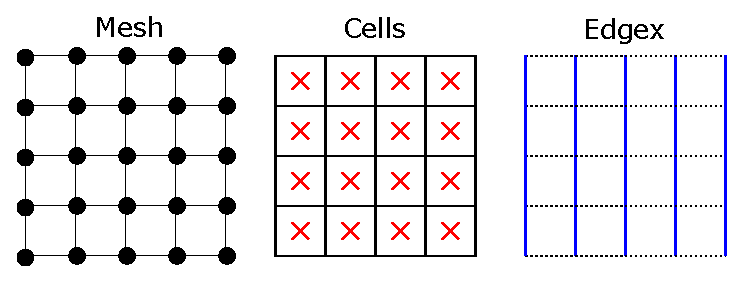
\includegraphics{./images/mesh.pdf}}
}\\
\hspace{10pt}
\subfloat[4-neighborhood stencil.\label{fig:ex1}]{
\resizebox{5cm}{!}{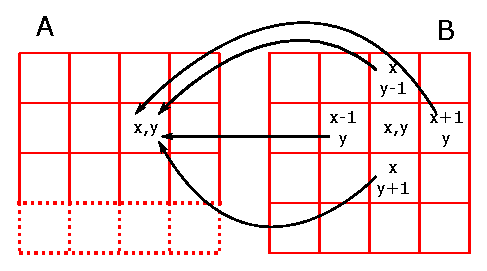
\includegraphics{./images/stencil1.pdf}}
}
\vspace{20pt}
\subfloat[4-neighborhood stencil.\label{fig:ex2}]{
\resizebox{5cm}{!}{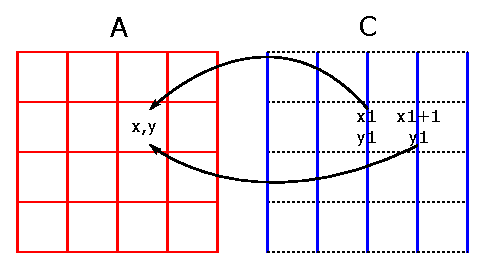
\includegraphics{./images/stencil2.pdf}}
}
\end{center}
\caption{(a) a Cartesian mesh and two kind of mesh entities, (b) an example of stencil kernel on cells, (c) an example of stencil kernel on two different entities of the mesh.}
\label{fig:gspmsp}
\end{figure}

A stencil program has been formally defined in this section. This formalism is used in the next Section to define two parallelization techniques of a multi-stencil program.

One can note that all definitions given in this section are not dependent from the topology of the mesh. This property will be kept in the rest of this paper to propose the mesh-agnostic MSL language.



%------------------------------------------------------------------------------
\section{Component-based parallelism}
\label{sect:component}
%----------------------------------------
%\subsection{Overview}
%----------------------------------------
This section describes both the projection of $\Gamma_{tsp}$ to
components, and the remaining needed components to execute a
multi-stencil application. Before those details the section gives an overview of
component models, and introduce the concepts of the Low Level Component Model \llc, which is used in this paper.


%----------------------------------------
\subsection{Component Model Overview}
%----------------------------------------
Component model is a domain of software
engineering~\cite{Szyperski:2002:CSB:515228}, which promotes code
re-use, separations of concerns, and thus maintainability. An
application is made of a set of components; a component being a kind of
black box representing an independent functionnality of the application, and which interacts only through its ports. A port specifies the services provided and required by the component.
%
With respect to high performance computing, some works have also shown
that component models can achieve the needed level of performance, and
scalability while also helping in application
portability~\cite{Bernholdt01052006, bigot:inria-00388508, UCHPC2015}

Many component models exist, each of them with its own specifications
and singularities. In distributed computing, well known component
models are CCM~\cite{corba:omg06} (CORBA Component Model), and
GCM~\cite{Baude} (Grid Component Model); in HPC, there are
CCA~\cite{Bernholdt01052006} (Common Component Architecture), and
\llc~\cite{l2c} (Low Level Component), for example.
%
As this work makes use of \llc, in particular for the experiments, let
introduce concepts of this component model with more details.

%----------------------------------------
\subsection{\llc}
%----------------------------------------

\llc is a minimalist \texttt{C++} based HPC-oriented component model
where a component extends the concept of class by specifying in its
interfaces the services that it offers ($provide$ ports) and that it
needs, either a single service instance ($use$ ports), or multiple
service instances ($use-multiple$ ports). Services are \texttt{C++}
interfaces. \llc also offers $MPI$ ports that enable components to
share MPI communicators. Components can also have attribute ports to
be configured.
%
As illustrated in Figures~\ref{fig:ports}, a $provide$ port is
represented with a white circle, a $use$
port with a black circle, a $use-multiple$ port by a black circle with
a white $m$ in it. MPI port are
connected with a black rectangle.

A classical \llc-based application is a static \emph{assembly} of
components made of instances of components and of connections between
component ports. Such an assembly is described in LAD, an XML
dialect~\cite{l2c}.

\begin{figure}[t]
\begin{center}
\subfloat[][\label{fig:2comp}]{
\begin{tikzpicture}[shorten >=1pt, node distance=2cm, on grid, auto]
   \node[component] (C) at (0,0) {$C_0$};
   \node[provide] (p) at (-1.5,0) {};
   \node[use] (u) at (1.5,0) {};
   \node[provide,right=1.5cm of u] (p1) {};
   \node[component,right=1.5cm of p1] (C1) {$C_1$};
   \node[use,right=1.5cm of C1] (um) {$m$};
 
  \path[-]
    (p) edge node {$p$} (C)
    (C.east) edge node {$u$} (u)
    (C1)  edge node {$v$} (um)
    (p1) edge node {$q$} (C1);
\end{tikzpicture}
}
\subfloat[][\label{fig:ass}]{
\begin{tikzpicture}[shorten >=1pt, node distance=2cm, on grid, auto]
   \node[component] (C) at (0,0) {$c_0$};
   \node[provide] (p) at (-1.5,0) {};
   \node[use] (u) at (1.5,0) {};
   \node[component,right=1.5 of u] (C1) {$c_1$};
   \node[use,right=1.5 of C1] (um) {$m$};
 
  \path[-]
    (p) edge node {$p$} (C)
    (C) edge node {$u$} (u)
    (C1)  edge node {$v$} (um)
    (u) edge node {$q$} (C1);
\end{tikzpicture}
}
\subfloat[][\label{fig:mpi}]{
\begin{tikzpicture}[shorten >=1pt, node distance=2cm, on grid, auto]
   \node[component] (C) at (0,0) {$c_2$};
   \node[provide] (p) at (-1.5,0) {};
   \node[mpi] (u) at (1.5,0) {};
   \node[component,right=1.5 of u] (C1) {$c_3$};
 
  \path[-]
    (p) edge node {$r$} (C)
    (C) edge node {$m_1$} (u)
    (u) edge node {$m_2$} (C1);
\end{tikzpicture}
}
\caption{Example of components and their ports representation. a) Component $c_0$ has a provide port ($p$) and a use port ($u$); Component $c_1$ has also a provide port ($q$) but also a use multiple port ($v$). b) A use port is connected to a (compatible) provide port. c) Component $c_2$ and $c_3$ shares an MPI communicator.}
\label{fig:ports}
\end{center}
\end{figure}

%% In the rest of this paper, when a required service of a \emph{use} (or \emph{use-multiple}) port is filled and linked to a \emph{provide} port in the comonent assembly, only the use port stay visible, as illustrated in Figure~\ref{fig:assembly}. As the use port is on the right of its component, and the provide port on the left, in a component assembly the component on the left uses the provide port of the component on the right.

%----------------------------------------
\subsection{MSCAC Runtime Overview}
%----------------------------------------

Figure~\ref{fig:mscac:assembly} gives an overview of the back-end component
assembly that is executed. As discusses in Section~\ref{sect:mscac},
there are different types of components. Components~\texttt{Driver},
\texttt{DriverApp}, and \texttt{Time} are always instanciated in the final component assembly; the input MSL file is not used by them except the component \texttt{Time} which uses the terminal \texttt{iteration} of the grammar. There is also a
single Component~\texttt{DDS} (the current version handles a single mesh
type). All these components are provided with the
compiler; dumping this part of the assembly is straightforward.

While Component~\texttt{DDS} is managing the structure of the mesh,
each data of the simulation is handled by a component of type
\texttt{Data}. Therefore, the compiler generates in the assembly as
many instances of such component as needed, from the \texttt{data}
section of an MSL program.

The last part of the assembly is the computation part. Each computation kernel is embedded in a kernel component, denoted K, which have to be written by the user and provided
to the compiler. A kernel component encapsulates a computations. To
access data, a kernel component is connected, by the compiler, to the adequate
\texttt{Data} components such that their ports name respect the names
given in the \texttt{data} section of MSL. We denote the fact that they may have
several use port by adding a star on the use port, as illustrated in Figure~\ref{fig:k}.
\begin{figure}
\begin{center}
\begin{tikzpicture}[shorten >=1pt, node distance=2cm, on grid, auto]
   \node[component] (k) at (0,0) {$K$};
   \node[provide] (p) at (-1.5,0) {};
   \node[use] (u) at (1.5,0) {};
   \node[right=0.2 of u] (star) {*};
 
  \path[-]
    (p) edge node {} (k)
    (k) edge node {} (u);
\end{tikzpicture}
\end{center}
\caption{Kernel component.}
\label{fig:k}
\end{figure}
  
%% In the computation part of the simulation a final component is needed,
%% the computation component, denoted K. This type of component
%% represents a single computation of the simulation, i.e. the
%% computation of a single output data (written) using a set of input
%% data (read). Using a \emph{use-multiple}, however, a list of component
%% is used and the explicit identification of each component to use is
%% lost. If for SEQ or PAR, the identification of components is not
%% usefull, it is usefull to manipulate data in a computation. For this
%% reason a computation component has as much \emph{use} ports as input
%% and output data to manipulate. We denote this in the bellow
%% representation as a star on the use port.

The rest of the computation part of the assembly contains the static parallel schedule
computed by MSC, \ie $\Gamma_{tsp}$. This is achieved through the use of
three specific components which manage the $P$, $S$, and $sync$
operations of $\Gamma_{tsp}$ as explained hereafter.

%----------------------------------------
\subsection{Control Components}
%----------------------------------------
The series-parallel tree decomposition $\Gamma_{tsp}$ represents the
control of the dependencies of the simulation. As a result to be able
to dump it to a component assembly it is needed to introduce what can
be called \emph{control components}. Those components can be used for
any case of simulation which increases code reuse between
simulations. A control component is composed of a single
\emph{provide} port linked to a single execution method, most of the
time called the \emph{go} method. We introduce three types of control
components represented in Figure~\ref{fig:ctrlcomponents}.

\begin{figure}[t]
\begin{tikzpicture}[shorten >=1pt, node distance=1cm, on grid, auto]
   \node[component] (seq) at (0,0) {$SEQ$}; \node[provide] (p) at
   (-1,0) {}; \node[use] (u) at (1,0) {$m$};
 
  \path[-]
    (p) edge node {} (seq)
    (seq) edge node {} (u);
\end{tikzpicture}
\hspace{\fill}
\begin{tikzpicture}[shorten >=1pt, node distance=1cm, on grid, auto]
   \node[component] (seq) at (0,0) {$PAR$};
   \node[provide] (p) at (-1,0) {};
   \node[use] (u) at (1,0) {$m$};
 
  \path[-]
    (p) edge node {} (seq)
    (seq) edge node {} (u);
\end{tikzpicture}
\hspace{\fill}
\begin{tikzpicture}[shorten >=1pt, node distance=1cm, on grid, auto]
   \node[component] (sync) at (0,0) {$SYNC$};
   \node[provide] (p) at (-1,0) {};
   \node[use] (u) at (1,0) {};
 
  \path[-]
    (p) edge node {} (sync)
    (sync) edge node {} (u);
\end{tikzpicture}
\\
a) Comp. SEQ
\hspace{\fill}
b) Comp. PAR
\hspace{\fill}
c) Comp. SYNC
\\
\caption{The three control components used by the back-end.}
\label{fig:ctrlcomponents}
\end{figure}

\begin{description}
\item[Sequence component (SEQ)] It is the direct representation of a sequence node of $\Gamma_{tsp}$. The role of this component is to call an ordered list of other components. Its interface contains an ordered \emph{use-multiple} port to be connected to the components to call in sequence.

\item[Parallel component (PAR)] It is the direct representation of a parallel node of $\Gamma_{tsp}$. The role of this component is to call simultaneously a set of other components. It offers a \emph{use-multiple} port to be connected to the components to call in parallel.
  
\item[Synchronization component (SYNC)]. It is the direct representation to an update leaf of $\Gamma_{tsp}$. The role of this component is to call the synchronization of a given data. It offers a \emph{use} port to be connected to the data to update.

\end{description}


%----------------------------------------
\subsection{Dump To Component Assembly}
%----------------------------------------
From $\Gamma_{tsp}$ and using the control components described above,
a direct dump can be done to a component assembly for an hybrid (data
and task) parallelization of a simulation. 
\fix{HC: ce qui suit est a changer avec la fusion du code de plusieurs composants}
However, it is also
possible to dump to a data parallelization only. In such a case the
computation of $\Gamma_{sync}$ is enough to generate the component
assembly. Actually a single SEQ component is thus needed and this
component is linked to all computations and synchronizations of
$\Gamma_{sync}$ directly.

Figure~\ref{fig:tsp:assembly} displays the assembly part corresponding to
$\Gamma_{tsp}$ of Figure~\ref{fig:tsp}. In this figure, the ports
linked to data (use and use-multiple ports of SYNC and K) are
represented but are not connected. Moreover, each computation
component is an instance of the component K presented before but using
the identification name of the computation in the MSL file.

\begin{figure*}[t]
\begin{center}
\begin{tikzpicture}[shorten >=1pt, node distance=2cm, on grid, auto]
   %seq0
   \node[component] (seq0) at (0,0) {$SEQ$};
   \node[provide] (seq0p) [left = 0.8cm of seq0] {};
   \node[use] (seq0u) [right = 1cm of seq0] {$m$};
   %c0
   \node[component] (c0) [right = 2cm of seq0u] {$c_0$};
   \node[use] (c0u) [right = 0.8cm of c0] {};
   \node[right=0.2 of c0u] (star) {*};
   %sync0
   \node[component] (sync0) [below = 1cm of c0] {$SYNC$};
   \node[use] (sync0u) [right = 1cm of sync0] {$m$};
   %c1
   \node[component] (c1) [below = 0.8cm of sync0] {$c_1^*$};
   \node[use] (c1u) [right = 0.8cm of c1] {};
   \node[right=0.2 of c1u] (star) {*};
   %par0
   \node[component] (par0) [below = 0.8cm of c1] {$PAR$};
   \node[use] (par0u) [right = 1cm of par0] {$m$};
  %seq1
   \node[component] (seq1) [right = 1cm of par0u] {$SEQ$};
   \node[use] (seq1u) [right = 1cm of seq1] {$m$};
   %par1
   \node[component] (par1) [right = 1cm of seq1u] {$PAR$};
   \node[use] (par1u) [right = 1cm of par1] {$m$};
  %c2
   \node[component] (c2) [right = 1cm of par1u] {$c_2$};
   \node[use] (c2u) [right = 0.8cm of c2] {};
   \node[right=0.2 of c2u] (star) {*};
  %sync1
   \node[component] (sync1) [below = 0.8cm of c2] {$SYNC$};
   \node[use] (sync1u) [right = 1cm of sync1] {$m$};
  %c4
   \node[component] (c4) [below = 0.8cm of par1] {$c_4^*$};
   \node[use] (c4u) [right = 0.8cm of c4] {};
   \node[right=0.2 of c4u] (star) {*};
  %c6
   \node[component] (c6) [below = 0.8cm of c4] {$c_6$};
   \node[use] (c6u) [right = 0.8cm of c6] {};
   \node[right=0.2 of c6u] (star) {*};
  %seq2
   \node[component] (seq2) [below = 2.5cm of seq1] {$SEQ$};
   \node[use] (seq2u) [right = 1cm of seq2] {$m$};
  %c3
   \node[component] (c3) [right = 1cm of seq2u] {$c_3$};
   \node[use] (c3u) [right = 0.8cm of c3] {};
   \node[right=0.2 of c3u] (star) {*};
  %c5
   \node[component] (c5) [below = 0.8cm of c3] {$c_5$};
   \node[use] (c5u) [right = 0.8cm of c5] {};
   \node[right=0.2 of c5u] (star) {*};
  %c7
   \node[component] (c7) [below = 0.8cm of par0] {$c_7$};
   \node[use] (c7u) [right = 0.8cm of c7] {};
   \node[right=0.2 of c7u] (star) {*};
  %sync2
   \node[component] (sync2) [below = 0.8cm of c7] {$SYNC$};
   \node[use] (sync2u) [right = 1cm of sync2] {$m$};
  %c8
   \node[component] (c8) [below = 0.8cm of sync2] {$c_8^*$};
   \node[use] (c8u) [right = 0.8cm of c8] {};
   \node[right=0.2 of c8u] (star) {*};

   \path[-]
   %seq0
    (seq0) edge node {} (seq0u)
    (seq0p) edge node {} (seq0)
   %c0
    (seq0u) edge node {} (c0)
    (c0) edge node {} (c0u)
    %sync0
    (seq0u) edge node {} (sync0.west)
    (sync0) edge node {} (sync0u)
    %c1
    (seq0u) edge node {} (c1)
    (c1) edge node {} (c1u)
   %par0
    (seq0u) edge node {} (par0.west)
    (par0) edge node {} (par0u)
  %seq1
    (par0u) edge node {} (seq1)
    (seq1) edge node {} (seq1u)
  %par1
    (seq1u) edge node {} (par1.west)
    (par1) edge node {} (par1u)
  %c2
    (par1u) edge node {} (c2)
    (c2) edge node {} (c2u)
  %sync0
    (par1u) edge node {} (sync1.west)
    (sync1) edge node {} (sync1u)
  %c4
    (seq1u) edge node {} (c4.west)
    (c4) edge node {} (c4u)
  %c6
    (seq1u) edge node {} (c6.west)
    (c6) edge node {} (c6u)
  %seq2
    (par0u) edge node {} (seq2.west)
    (seq2) edge node {} (seq2u)
  %c3
    (seq2u) edge node {} (c3)
    (c3) edge node {} (c3u)
  %c6
    (seq2u) edge node {} (c5.west)
    (c5) edge node {} (c5u)
  %c6
    (seq0u) edge node {} (c7.west)
    (c7) edge node {} (c7u)
  %sync2
    (seq0u) edge node {} (sync2.west)
    (sync2) edge node {} (sync2u)
  %c8
    (seq0u) edge [bend right] node {} (c8.west)
    (c8) edge node {} (c8u)
   ;
\end{tikzpicture}
\caption{Component assembly representing the computation part generated from $\Gamma_{tsp}$ of Figure~\ref{fig:tsp}.}
\label{fig:tsp:assembly}
\end{center}
\end{figure*}

%----------------------------------------

%------------------------------------------------------------------------------
\section{Component Stencil Model}
\label{sect:csm}
%-------------------------------------
\subsection{Phase, group and kernel}
Using the formalism described in Sections~\ref{sect:formalism} and~\ref{sect:component}, the following definitions are given for the solution.

\medskip
\begin{mydef}
For a stencil program $\mathcal{P}(\mathcal{M},\Delta,\Gamma,\mathcal{T})$, a \emph{phase} $\Phi \subset \Gamma$ is a subset of ordered computations $\{c_0,...,c_{n-1}\} \in \Gamma$ such that $\forall 0 \leq i,j \leq n-1, \nexists c_i,c_j \in \Phi$, which verifies $c_i \ll c_j$.
\end{mydef}

One can notice, however, that in a phase $Phi$ of a stencil program it is possible to have a pair $c_i,c_j \in \Phi$, which verifies $c_i<c_j$. As a result, a phase is equivalent to a sequence of computations $SEQ$. The set of phases of a stencil program are ordered and a synchronization is needed between two different \emph{phases} of a stencil program $\mathcal{P}$. In other terms for two phases $\Phi_1$ and $\Phi_2$ $\exists c_i \in \Phi_1, c_j \in \Phi_2$ such that $c_i \ll c_j$. If $m$ is the number of stencil computations in a phase $\Phi_i$ among $n$ total computations, the synchronizations of $\Phi_i$ are applied on $\bigcup_{j=0}^{m-1}R_j$. 

Instead of introducing an additional definition for the equivalent of $SSEQ$, and because $sequence(sequence(a,b),sequence(c,d))=sequence(a,b,c,d)$, synchronizations needed by a new phase are commputed inside the Phase itself before computations. A phase component is defined as
\begin{equation}
Phase(\{provide,use-multiple, synchronization\},\{phase\}).
\end{equation}
 The function $phase$ performs the needed synchronizations before to use each component of the sequence

\begin{algorithm}[H]
 synchronizations\\
 \ForAll{component $cp$ to use}{
 use the provide interface of $cp$
 }
 \caption{phase function}
 \end{algorithm}

\begin{mydef}
For a stencil program $\mathcal{P}(\mathcal{M},\Delta,\Gamma,\mathcal{T})$, a \emph{group} $\mathcal{G} \subset \Gamma$ is a subset of unordered computations $\{c_0,...,c_{n-1}\}$ such that $\forall 0 \leq i,j \leq n-1, \nexists c_i,c_j \in \mathcal{G}$, which verifies $c_i<c_j$.
\end{mydef}

Thus, a dependency exists between two different \emph{groups} of a stencil program $\mathcal{P}$, but the computations inside a \emph{group} are unordered, without dependencies. As a result, the Group component is defined as $PAR$
\begin{equation}
Group(\{provide,use-multiple\},\{group\}),
\end{equation}
 where the function $group$ creates a thread for each component to use, and join all threads at the end.

\begin{algorithm}[H]
 \ForAll{component $cp$ to use}{
 create thread $t$
 $t$ uses the provide interface of $cp$
 }
 join all threads
 \label{alg:par}
 \caption{group function}
 \end{algorithm}

\begin{mydef}
For a stencil program $\mathcal{P}(\mathcal{M},\Delta,\Gamma,\mathcal{T})$, a \emph{kernel} $\mathcal{K} \subset \Gamma$ is a subset of unordered computations $\{c_0,...,c_{n-1}\}$ such that $\forall 0 \leq i,j \leq n-1, \nexists c_i,c_j \in \mathcal{K}$, which verifies $c_i<c_j$, and where $\forall i,j<n, D_i=D_j$.
\end{mydef}

\medskip
Thus, a \emph{kernel} could contains $n$ computations $\{c_0,...,c_{n-1}\}$, but handles a single space loop in a coarser computation $c'$ such that $c'(\bigcup_{i=0}^{n-1}R_i,\bigcup_{i=0}^{n-1}w_i,D,\{e_0,...,e_{n-1}\})$. This definition differs from the component $K$ described in this section as a kernel could contains more than one computation if the space domain is the same. This definition of a kernel improves performances as the memory bandwidth is better used. A kernel component if defined as
\begin{equation}
Kernel(\{provide\},\{kernel\}).
\end{equation}
 The function $kernel$ performs the set of numerical computations

\begin{algorithm}[H]
 \ForAll{elements $d$ in $D$}{
 $w(d)=e_1(R(d),R(\mathcal{N}(d)))$\\
 $w(d)=e_2(R(d),R(\mathcal{N}(d)))$\\
 ...
 }
 \caption{kernel function}
 \end{algorithm}

\medskip
The component assembly of the computations of a mesh-based numerical simulation using phase, group and kernel components is represented in the Figure~\ref{phgpk}. This assembly is equivalent to the one presented in the Figure~\ref{approx}, but $SSEQ$ and $SEQ$ are fusionned in $phase$, and the component $kernel$ is bit different from $K$.

%---------
\begin{figure}[h!]
\begin{center}
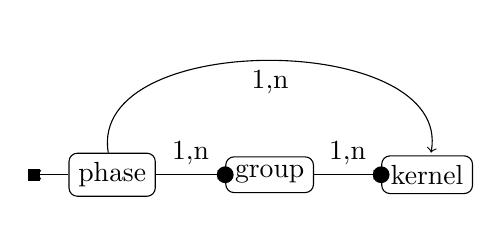
\begin{tikzpicture}[shorten >=1pt, node distance=2cm, on grid, auto]
   \node[component] (phase) at (0,0) {phase};
   \node[component] (group) [right=of phase] {group};
   \node[component] (kernel) [right=of group] {kernel};
 
  \path[->]
             (phase)  edge  [connection]               node           {1,n}   (group)
                      edge [mpiconn] node {} (-1,0)
             (group)   edge [connection]          node       {1,n}   (kernel)
             (phase)   edge [bend left=100,connection]   node  [swap]   {1,n}   (kernel);
\end{tikzpicture}
\caption{General assembly proposed in our solution}
\label{phgpk}
\end{center}
\end{figure}

This component assembly of computations can be, by definition, extracted from an ordered list of typed computations $s(R,w,D,e,\mathcal{N})$ or $l(R,w,D,e)$. $R$, $w$ and $D$ are used to build Phases, Groups and Kernels, while $e$ and $\mathcal{N}$ are used inside the Kernel components. As a result, we can define a function $\lambda$ to build the computation assembly
\begin{equation}
\lambda : list_o(c(R,w,D,e)) \rightarrow \alpha ({{Phase},{Group},{Kernel}},L,R)
\end{equation}

%-------------------------------------
\subsection{Overall assembly}

\paragraph{The SIPSim model.} The SIPSim model~\cite{} is a model which proposes a systematic way to create an SPMD implicit parallelism solution for mesh-based numerical simulations through four concepts. The first concept is a \textit{Distributed Data Structure} (DDS), which represents the distributed mesh. Thus, the DDS manages a domain decomposition, or more broadly a graph partitioning problem which balances the number of elements on available resources, and which tries to minimize the number of needed synchronizations between resources. It has to be noticed that this particular task could be managed by an external graph partitionner. In addition to this, the DDS also has to offer an efficient access to an element of a mesh and to its neighborhood. The second concept is the \textit{Distributed Property Map} (DPMap), which is responsible to map a quantity to simulate (a data) onto the distributed mesh. The third concept is an \textit{applicator}, which is responsible for applying a set of synchronizations before a set of numerical computations written by the user (also called operations). Finally, the last concept contains the \textit{interfaces} needed to write an operation in a sequential programming style while using DPMaps mapped onto the DDS. Those interfaces are directly linked to the type of DDS used.

\paragraph{CSM overall assembly.} From the SIPSim model, CSM uses the concept of DDS and DPMap and transforms them in components to build the overall component assembly. The implementation of those components are not described in this paper, and it is possible to imagine an adhoc implementation in simple cases, as a Cartesian mesh, or existing external implementations (libraries) in more complex cases. This choice is an implementation choice and will be compatible with CSM. In addition to those two new components, the concept of \textit{interface} of the SIPSim model has to be kept to write the implementation of the expressions $e$ of the numerical computations on distributed data structures. But this concept is not needed as a component. It could be provided by the DDS itself or it could be introduced as a header file for example.

The overall assembly produced by the model is presented in the Figure~\ref{csmassembly}. First, the component \textit{DDS} and the component \textit{Data}, which corresponds to the DPMap concept of the SIPSim model, are introduced in the assembly with the same functionnality than described above. 

Second, one can notice that the assembly described in the previous Figure~\ref{phgpk} is, of course, inserted in the overall assembly. However, even if the \textit{Phase} component is still responsible for starting a set of synchronizations, those synchronizations are in fact performed by the \textit{Connector} component. Actually, the \textit{Phase} component uses the data concerned by its synchronizations, and then each data uses the \textit{Connector}, which finally performs the synchronizations. As a result, the \textit{Connector} component can be implemented with threads, or with MPI, without the modification of \textit{Phase} and \textit{Data} components. This is a separation of concerns between the data of the simulation and the parallelization strategy which increases the portability of the application. This strategy has been more described in the paper~\cite{}. 

The third important point to notice is the introduction of the component \textit{Time} which is responsible for the time iteration steps of the simulation. To establish the end of time steps, most of the time a convergence function is computed on data, but it also happens that a fix number of iterations is precised. For this reason, the instanciation of the component \textit{Convergence} is optional. The \textit{Driver} component starts the simulation and launches the initialization of the DDS, and the \textit{DrApp} component starts the initialization of the data and also the time loop of the simulation. Finally, the \textit{Initializer} component is linked to the initialization of data (read a file format, default value, or numerical computation). The computation components, specific to each simulation, are \textit{Kernel} and \textit{Convergence}, and to perform numerical expressions $e$ those components have to be connected to the Data of each $R$ and $w$.

%---------
\begin{figure}[h!]
\begin{center}
\begin{tikzpicture}[shorten >=1pt, node distance=2cm, on grid, auto]
   \node[component] (phase) at (0,0) {Phase};
   \node[component] (group) [right=of phase] {Group};
   \node[component] (kernel) [right=of group] {Kernel};
   \node[component] (init) [above=1.5cm of group] {Initializer};
   \node[component] (data) [above=1.5cm of phase] {Data};
   \node[component] (time) [left=of phase] {Time};
   \node[component] (drapp) [above=1.5cm of time] {DrApp};
   \node[dcomponent] (conv) [left=of time] {Convergence};
   \node[component] (dr) [above=1.5cm of drapp] {Driver};
   \node[component] (dds) [above=1.5cm of data] {DDS};
   \node[component] (connec) [above=1.5cm of init] {Connector};
 
  \path[->]
  	(dr)		edge  [connection]	node	{}	(dds)
  	(dr)		edge  [connection]	node	{}	(drapp)
  	(drapp)		edge  [connection]	node	{1,n}	(data)
  	(drapp)		edge  [connection]	node	{}	(time)
  	(data)  	edge  [connection]	node	{}	(dds)
  	(data)  	edge  [connection]	node	{}	(connec)
  	(connec)	edge  [connection]	node	{}	(dds)
  				edge  [mpiconn]		node	{}	(4,3)
  	(data)		edge  [connection]	node	{1,n}	(init)
  	(time)		edge  [connection]	node	{}	(conv)
  	(time)		edge  [connection]	node	{1,n}	(phase)
  	(phase)		edge  [connection]	node	{1,n}	(data)
  	(phase)		edge  [connection]	node	{1,n}	(group)
  	(phase)		edge  [bend right=50,connection]   node  [swap]   {1,n}   (kernel)
  	(group)		edge  [connection]	node	{1,n}	(kernel)
  	(kernel)	edge  [connection]	node	{1,n}	(data)
  	(conv)	edge  [connection,dashed]	node	{1,n}	(data);
\end{tikzpicture}
\caption{Overall assembly of the Component Stencil Model.}
\label{csmassembly}
\end{center}
\end{figure}

This overall assembly can be compiled from a set of sequential and descriptive information. First an unordered list of data is needed. A data is defined as
\begin{equation}
data(init_f,E_i,type)
\end{equation}
, where $init_f$ is the function to initialize the data (in the Initializer component), $Ei$ is the set of elements of the mesh on which the data is applied, and $type$ is the actual type of data ($int$, $double$ etc.).

The second needed information is the description of the mesh to use as
\begin{equation}
mesh(type,dimension,size)
\end{equation}
, where $type$ of is the topology of the mesh (for example Cartesian or k-sided unstructured meshes), $dimension$ is the dimension of the mesh, and $size$ is the size of the mesh.

As a result, we can define a function $\Lambda$ to build the overall simulation assembly of the Figure~\ref{csmassembly} as
\begin{equation}
\Lambda : list_o(c(R,w,D,e)) \times list(data(init_f,E_i,type)) \times mesh(type,dimension,size) \rightarrow \alpha (\mathcal{C},L,R)
\end{equation}

The needed information of the function $Lambda$ are typically produced by numericians who try to solve a set of partial differential equations by existing numerical methods, by a combination of methods, or by their own methods. Once the parallel assembly $\alpha$ is created, the engineer or a numerican developper of the lab can write the set of numerical computation components $Kernel$, the set of $Initializer$ components, and eventually the $Convergence$ component. All those components are written with an imperative sequential programming style using the interfaces linked to the DDS. As a result, multiple levels of separation of concerns are introduced. First the separation of concerns between the numerician and the person in charge of the implementation, and second the separation of concerns between the implementation and the parallelization of the simulation, which is generated.

%\paragraph{Evaluation.}
% for different kind of mesh

%------------------------------------------------------------------------------
\section{Component Stencil Language}
\label{sect:csl}
%-------------------------------------
\subsection{CSL language}

%-------------------------------------
\subsection{CCSL compiler}

%-------------------------------------
\subsection{Performance evaluation}
%------------------------------------------------------------------------------
\section{Related work}
\label{sect:rel}
%------------------------------------------------------------------------------
\section{Conclusion}
\label{sect:concl}
%------------------------------------------------------------------------------
\label{sect:bib}
\bibliographystyle{abbrvnat}


\tableofcontents

\end{document}
\endinput
%%
%% End of file `squelette-rr.tex'.
